\chapter{Exercise 09}
\extitle{Confusion Matrix}
%%******************************************************************************%
%                                                                              %
%                                 Interlude                                    %
%                         for Machine Learning module                          %
%                                                                              %
%******************************************************************************%

% ============================================== %
\section*{Interlude - Lost in Overfitting}
% ---------------------------------------------- %

The two previous exercises lead you, dear reader, to a very dangerous territory: the realm of \textbf{overfitting}.\\
You did not see it coming but now, you are in a bad situation...\\
\\
By increasing the polynomial degree of your model, you increased its \textbf{complexity}.  
Is it wrong?
Not always.
Some models are indeed very complex because the relationships they represent are very complex as well.\\
\\
But, if you look at the plots for the previous exercise's \textit{best model}, you should feel that something is wrong...\\
\\
% ============================================== %
\section*{Interlude - Something is rotten in the state of our model...}
% ---------------------------------------------- %
Take a look at the following plot. 

\begin{figure}[!h]
    \centering
    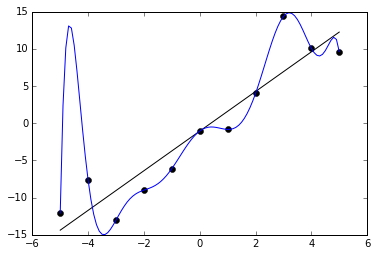
\includegraphics[scale=0.6]{assets/overfitt.png}
    \caption{Overfitting hypothesis}
\end{figure}

You can see that the prediction line fits each data point perfectly, but completely misses out on capturing the relationship between $x$ and $y$ properly.
And now, if we add some brand new data points to the dataset, we see that the predictions on those new examples are way off.

\begin{figure}[!h]
    \centering
    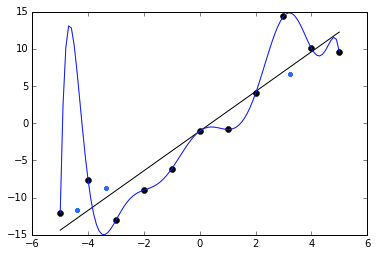
\includegraphics[scale=0.6]{assets/overfitt_with_dots.png}
    \caption{Generalization errors resulting from overfitting}
\end{figure}
This situation is called overfitting, because the model is doing an excessively good job at fitting the data.
It is literally bending over backward to account for the data's mini details.
But most of the data's irregularities are just noise, and they should in fact be ignored.
So because the model overfits, it can't generalize to new data.

% ============================================== %
\section*{Interlude - The training set, the test set, and the happy data scientist}
% ---------------------------------------------- %
To be able to detect overfitting, \textbf{you should always evaluate your model on new data}.\\
\\
New data means, data that your model hasn't seen during training.\\
\\
It's the only way to make sure your model isn't \textit{recalling}.
To do so, now and forever, you must always divide your dataset in (at least) two parts: one for the training, and one for the evaluation of your model.
%\newpage
\turnindir{ex09}
\exnumber{09}
\exfiles{confusion\_matrix.py}
\exforbidden{None}
\makeheaderfilesforbidden

% ================================= %
\section*{Objective}
% --------------------------------- %
Manipulation of confusion matrix concept.\
The goal of this exercise is to reimplement the function \texttt{confusion\_matrix} available in \textbf{sklearn.metrics} and to learn what does the confusion matrix represent.

% ================================= %
\section*{Instructions}
% --------------------------------- %
For the sake of simplicity, we will only ask you to use three parameters.
Be careful to respect the order, true labels are rows and predicted labels are columns:

\begin{center}
  \begin{tabular}{|c|c|c|c|}
    \cline{3-4}
    \multicolumn{2}{c|}{\multirow{2}{*}{}}  & \multicolumn{2}{|c|}{predicted labels} \\ \cline{3-4}
    \multicolumn{2}{c|}{}       & label 1 & label 2 \\
    \hline
    \multirow{2}{*}{true label} & label 1 &         &         \\
    \cline{2-4}
                                & label 2 &         &         \\
    \hline
  \end{tabular}
\end{center}

In the \texttt{confusion\_matrix.py} file, write the following function as per the instructions below:

\begin{minted}[bgcolor=darcula-back,formatcom=\color{lightgrey},fontsize=\scriptsize]{python}
def confusion_matrix_(y_true, y_hat, labels=None):
    """
    Compute confusion matrix to evaluate the accuracy of a classification.
    Args:
        y_true: numpy.ndarray for the correct labels
        y_hat: numpy.ndarray for the predicted labels
        labels: Optional, a list of labels to index the matrix.
                This may be used to reorder or select a subset of labels. (default=None)
    Returns: 
        The confusion matrix as a numpy ndarray.
        None on any error.
    Raises:
        This function should not raise any Exception.
    """
    ... Your code ...
\end{minted}


% ================================= %
\section*{Examples}
% --------------------------------- %
\begin{minted}[bgcolor=darcula-back,formatcom=\color{lightgrey},fontsize=\scriptsize]{python}
import numpy as np
from sklearn.metrics import confusion_matrix

y_hat = np.array([['norminet'], ['dog'], ['norminet'], ['norminet'], ['dog'], ['bird']])
y = np.array([['dog'], ['dog'], ['norminet'], ['norminet'], ['dog'], ['norminet']])

# Example 1: 
## your implementation
confusion_matrix_(y, y_hat)
## Output:
array([[0 0 0]
       [0 2 1]
       [1 0 2]])
## sklearn implementation
confusion_matrix(y, y_hat)
## Output:
array([[0 0 0]
       [0 2 1]
       [1 0 2]])

# Example 2:
## your implementation
confusion_matrix_(y, y_hat, labels=['dog', 'norminet'])
## Output:
array([[2 1]
       [0 2]])
## sklearn implementation
confusion_matrix(y, y_hat, labels=['dog', 'norminet'])
## Output:
array([[2 1]
       [0 2]])
\end{minted}

\section{Optional part}

\subsection{Objective(s):}

For a more visual version, you can add an option to your previous confusion\_matrix\_ function to return a \texttt{pandas.DataFrame} instead of a numpy array.

\subsection{Instructions:}

In the \texttt{confusion\_matrix.py} file, write the following function as per the instructions below:

\begin{minted}[bgcolor=darcula-back,formatcom=\color{lightgrey},fontsize=\scriptsize]{python}
def confusion_matrix_(y_true, y_hat, labels=None, df_option=False):
    """
    Compute confusion matrix to evaluate the accuracy of a classification.
    Args:
        y_true: a numpy.ndarray for the correct labels
        y_hat: a numpy.ndarray for the predicted labels
        labels: optional, a list of labels to index the matrix. This may be used to reorder or select a subset of labels. (default=None)
        df_option: optional, if set to True the function will return a pandas DataFrame instead of a numpy array. (default=False)
    Returns: 
        Confusion matrix as a numpy ndarray or a pandas DataFrame according to df_option value.
        None on any error.
    Raises:
        This function should not raise any Exception.
    """
    ... Your code ...
\end{minted}

\section{Examples:}

\begin{minted}[bgcolor=darcula-back,formatcom=\color{lightgrey},fontsize=\scriptsize]{python}
import numpy as np
y_hat = np.array(['norminet', 'dog', 'norminet', 'norminet', 'dog', 'bird'])
y = np.array(['dog', 'dog', 'norminet', 'norminet', 'dog', 'norminet'])

# Example 1: 
confusion_matrix_(y, y_hat, df_option=True)
# Output:
           bird  dog  norminet
 bird         0    0         0
 dog          0    2         1
 norminet     1    0         2

# Example 2:
confusion_matrix_(y, y_hat, labels=['bird', 'dog'], df_option=True)
# Output:
           bird  dog
 bird         0    0
 dog          0    2
\end{minted}

\info{
  If you fail this exercise on your first attempt, Norminet will curse you forever.
  Yeah, you'd better do it right or you are in trouble my friend, big trouble!
}